% Week 4 实验周报 —— 编译方式:XeLaTeX
\documentclass[11pt]{ctexart}
\usepackage[a4paper, margin=2.5cm]{geometry}
\usepackage{amsmath}
\usepackage{booktabs}
\usepackage{graphicx}
\usepackage{hyperref}
\usepackage{enumitem}
\setlist{nosep}

\title{\textbf{Chooser Option 定价项目 —— 第 4 周实验报告}\\
\large Baseline Model Performance Evaluation}
\author{佟铸城 (Zhucheng Tong)}
\date{2026 年 8 月 11 日}

\begin{document}
\maketitle

\section{本周目标}
完成 Week 4 三项交付物:(1) 含误差指标(MAE/RMSE)的模型验证报告;(2) 性能基准文档(供第 5--6 周 ML 对比);(3) 优化且注释完善的 BSM 代码。

\section{完成工作}
\begin{enumerate}
  \item \textbf{三层评估框架}:实现正确性(MC vs 闭式解,多种子 MAE/RMSE)、假设失效(真实数据滚动校准 vs 事后真值)、选择规则代价(真实利率状态复检)——详见《基线模型验证与性能基准报告》;
  \item \textbf{逐日滚动定价}:1310 个交易日(2019-10 至 2024-12),每日 ATM chooser,参数全部来自第 2 周特征管道($r$=期限匹配国债、$q$=TTM 股息率、$\sigma$=四种回望估计器);事后真值用期权存续期内实际实现的波动率(数据管道自动延伸的 2025 年数据在此派上用场);
  \item \textbf{基准表}(\texttt{docs/week4/baseline\_metrics.csv}):最佳回望校准(EWMA)MAE \$9.44 / 相对 35.3\%,即 ML 起跑线;
  \item \textbf{代码}:定价全程 numpy 向量化(1310 天 $\times$ 5 变体约 2 毫秒);走查脚本内置四项独立审计断言。
\end{enumerate}

\section{核心发现}
\begin{enumerate}
  \item \textbf{常数波动率假设的代价约为价格的 35\%}(1 年期 ATM chooser,最佳回望校准),且——
  \item \textbf{失效模式取决于估计器的记忆长度}:快估计器(21日/EWMA)在\textbf{恐慌期}失效(追高后市场均值回复,MAE 11.4/10.8 vs 平静期 9.3/9.0);慢估计器(252日)在\textbf{危机后的平静期}失效(窗口拖尾,2021 年 MAE \$10.34 vs 21 日的 \$6.13)。没有单一窗口全状态占优——这是第 5 周 ML 有条件组合多窗口与前瞻 VIX 特征的直接动机;
  \item \textbf{不可预见性的边界}:2019 年尾段误差(\$31.8)源于存续窗口内的 COVID 崩盘,任何回望方法都无法预见——ML 的合理目标是改善可预测的波动率动态(聚集/均值回复/状态切换),而非黑天鹅;
  \item \textbf{W3 伏笔回收}:论文 moneyness 规则的代价在真实数据上随利率放大(2021-06 低利率 14.4bp $\to$ 2023-10 高利率 32.2bp,约 2.2 倍),本项目全程采用理性规则;
  \item \textbf{EWMA 的单日跳变过敏}:2024-11 大选日 JPM $+11.5\%$ 令 EWMA 定价短暂冲高——"跳变 vs 持续状态"的区分是 ML 特征可着力之处。
\end{enumerate}

\begin{figure}[h!]
\centering
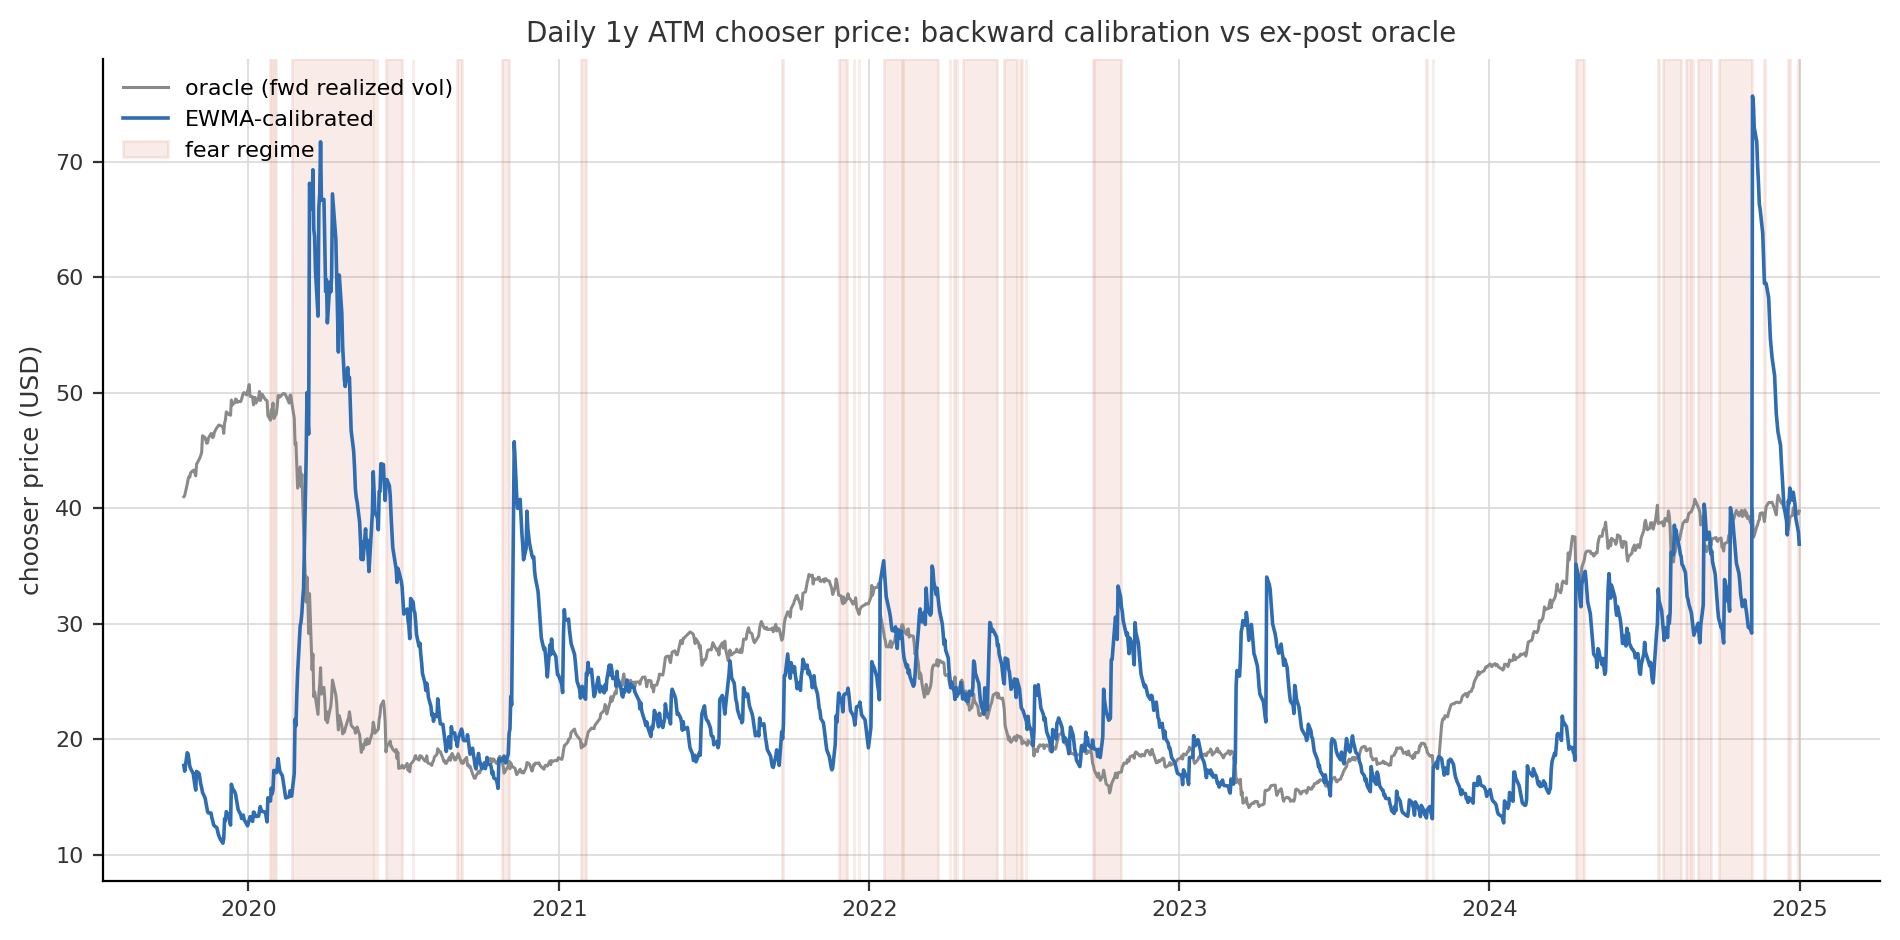
\includegraphics[width=0.9\textwidth]{../../docs/week4/figures/rolling_price.png}
\caption{逐日定价:回望校准(蓝) vs 事后真值(灰),阴影为恐慌状态}
\end{figure}

\section{扩展指标与加权综合评分(v2,应导师要求新增)}
在 MAE/RMSE 之外扩充至\textbf{八项指标}(MedAE、Bias、P95AE、分状态最差 MAE、$R^2$、Hit10),并构建加权综合分:各指标统一为``越小越好''后除以 EWMA 基线值、按权重(平均精度 0.35 / 尾部稳健 0.30 / 偏差 0.10 / 解释力 0.10 / 可用率 0.15)加权求和——\textbf{综合分 $<1$ 即优于基线},第 5--6 周 ML 沿用同一把尺。基线结果的两个要点:(1) 四个回望基线综合分 0.98--1.07,实质打平且排名对权重敏感(附四种权重方案的敏感性检验;21d 在所有方案下恒为末位),各窗口只是在``平均精度 vs 尾部稳健''间取舍——进一步佐证无单一回望方案可用;(2) \textbf{所有基线对 oracle 价格的 $R^2$ 为负}(约 $-1.1$),即解释力不如常数均值预测——常数波动率失效的最尖锐表述,也为 ML 设定了第一目标:先把 $R^2$ 转正。完整定义、公式与权重理由见《基线模型验证与性能基准报告》第 5 节;指标模块 \texttt{src/metrics.py} 为可复用组件。

\section{实验记录}
自检机制的一个实例值得记录:审计断言原假设"所有估计器恐慌期误差 $>$ 平静期",被 252 日估计器\textbf{证伪}——追查后发现这不是 bug 而是拖尾效应的真实结构,遂将其转为经验证的发现写入报告,并把断言改为"快估计器恐慌期更差 + 慢估计器平静期更差"的结构性检验。假设被数据推翻的时刻往往是发现的入口。

\section{下周计划(Week 5:ML 模型设计与实现)}
\begin{enumerate}
  \item 路线 A:以特征集预测未来波动率(RF/XGBoost/LSTM),预测值代入 BSM 定价,与基准表对比;
  \item 路线 B:端到端监督定价(以 oracle 价为标签)的框架搭建;
  \item 70/15/15 时序切分(杜绝前视偏差),训练集截至约 2023 年;
  \item 特征取舍参照第 2 周重要性分析(VIX 系前瞻特征为先验重点)。
\end{enumerate}

\end{document}
